\section{Exploring the Data}
\label{sec:Exploring the Data}

\subsection{Relationships Dataset}
\label{subsec:Relationships Dataset}

\begin{figure}[H]
\begin{center}

        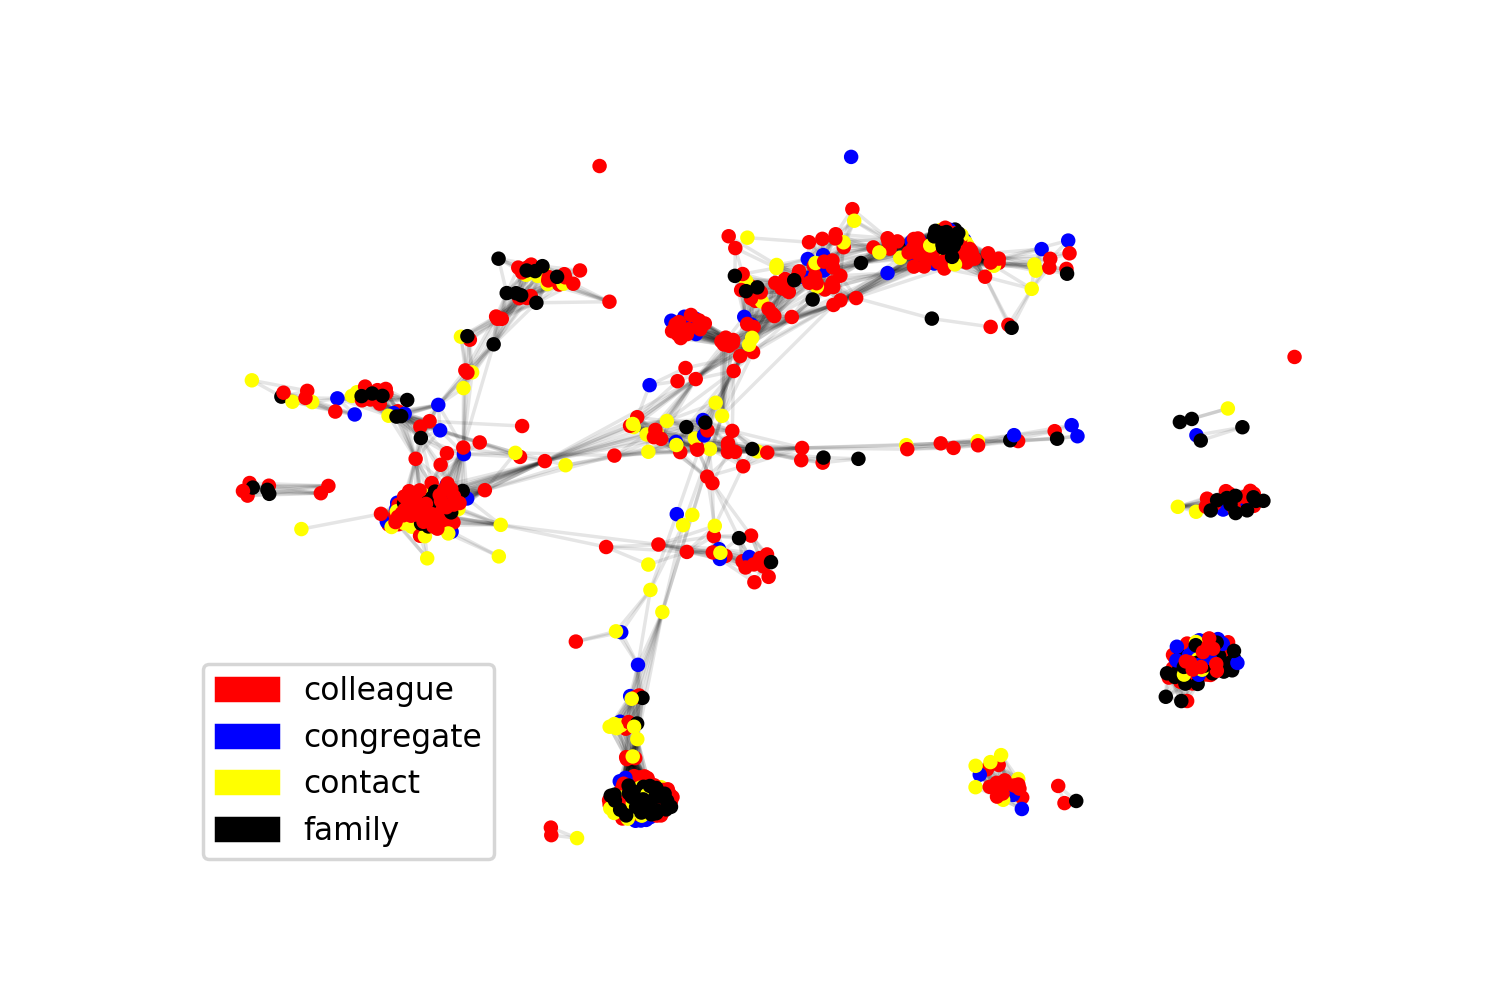
\includegraphics[width=.5\textwidth]{graphRel.png}
        \label{fig:graphLoc}
        \caption{Terrorist relation dataset graph. The colouring of each node is related to the type of relation that corresponds to it}
        
\end{center}
\end{figure}


This dataset is the line-graph of a network of relationship between terrorists. Each node represents a connection between two individuals and each edge an individual. 
The label of each note relates to the nature of the relation between the two individual. It is one of the following four: 
Family - congregate - colleague -contact.
Two nodes are connected if they share one individual.

Our interest was to investigate the proprieties of the line graph as a relational network. As "original paper on dataset" mentions, an organisation need interpersonal connection to function and studying the structure of the social organisation could yield valuable insight.
"Paper on line graph for social networks" found that on the basis of a study of an online social network, a social network could be well approximated by the line graph of a scale free network. If that propriety can be verified by our dataset, then we could gain information from the original graph from which the line graph originates.

\label{subsec:Proprieties of the graphs}
Social sciences studies have shown that social/relationship networks have the particularities of homophily and transitivity.
Logically if $a$ \& $b$ are friends and $c$\& $b$ are also, the it is more likely that $a$ \& $c$ are friends than not. This mathematically translates to:
\begin{equation}
	a \sim b \text{ and } b \sim c \text{ then } a \sim c
\end{equation}

As a first research question we will try to verify that our dataset derives from a scale-free network, implying that the graph that generated the relationship dataset have proprieties similar to social networks.
By creating a scale-free network and making its line graph, we compared the degree distribution of the relationship dataset we were able to show that.

\begin{figure}[H]
\begin{center}
    \begin{subfigure}[b]{0.45\textwidth}
        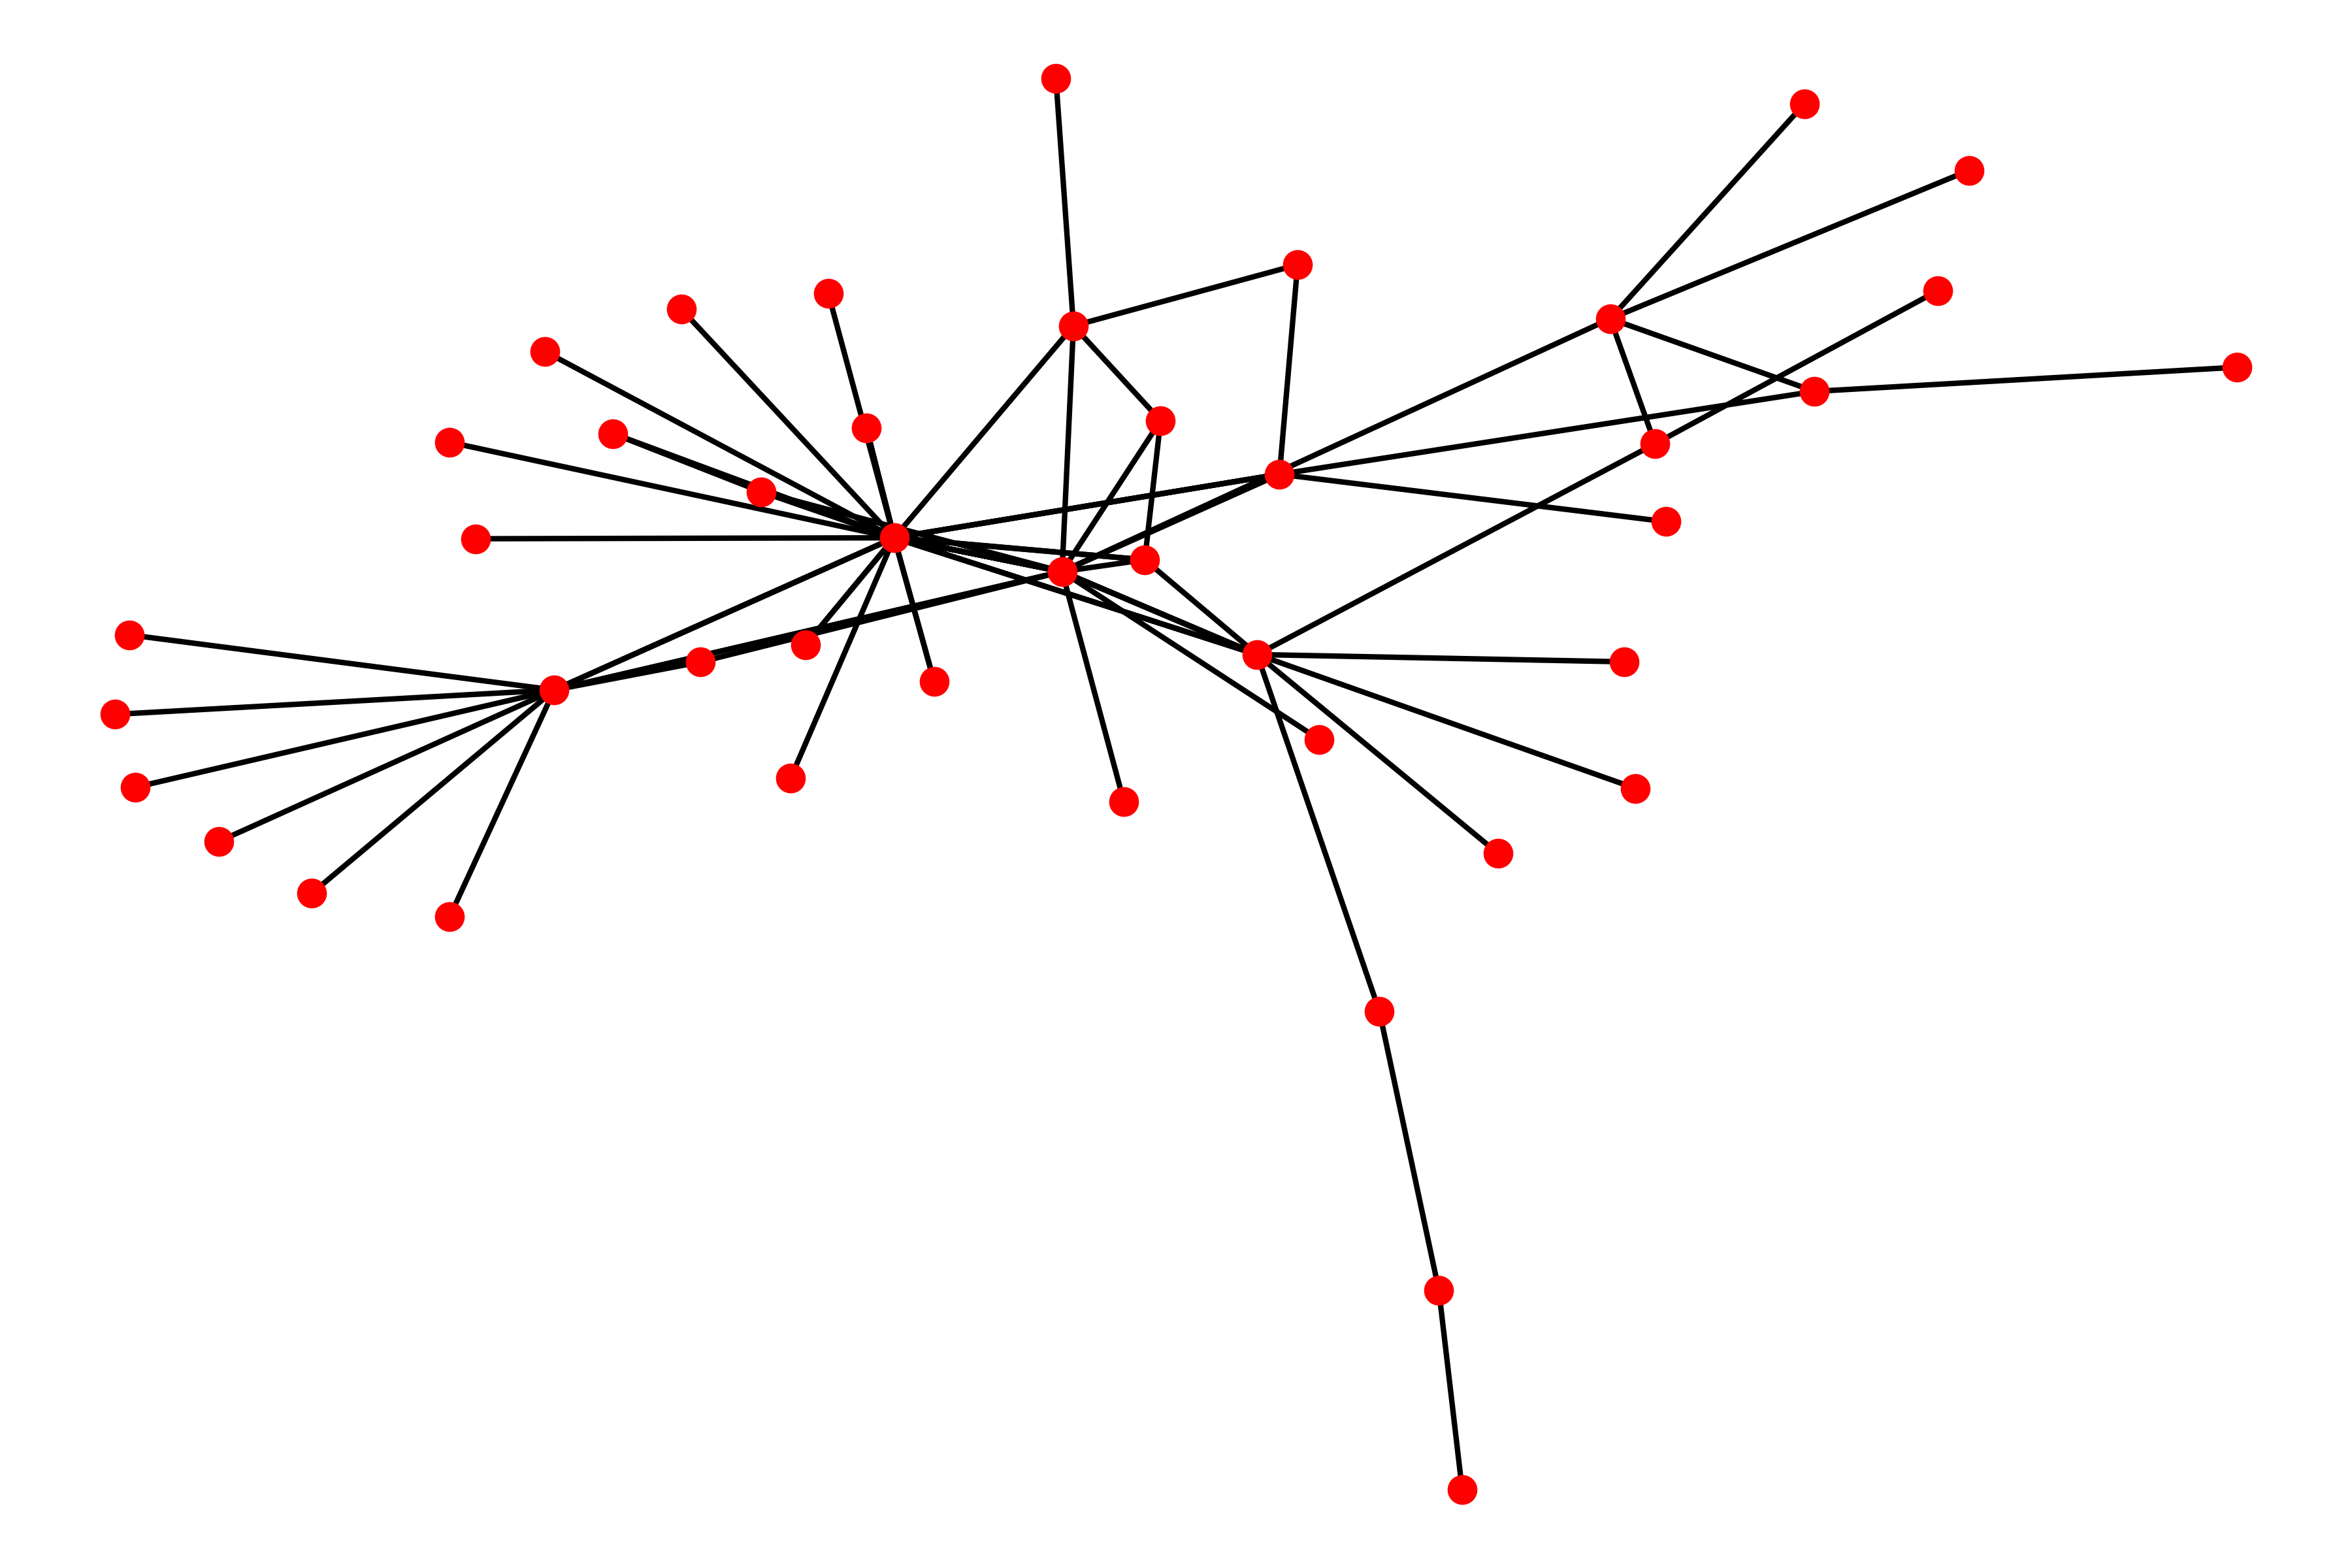
\includegraphics[width=\textwidth]{graphScaleFree.png}
        \caption{Scale free network}
        \label{fig:Scalefree}
    \end{subfigure}
    ~
    \begin{subfigure}[b]{0.45\textwidth}
        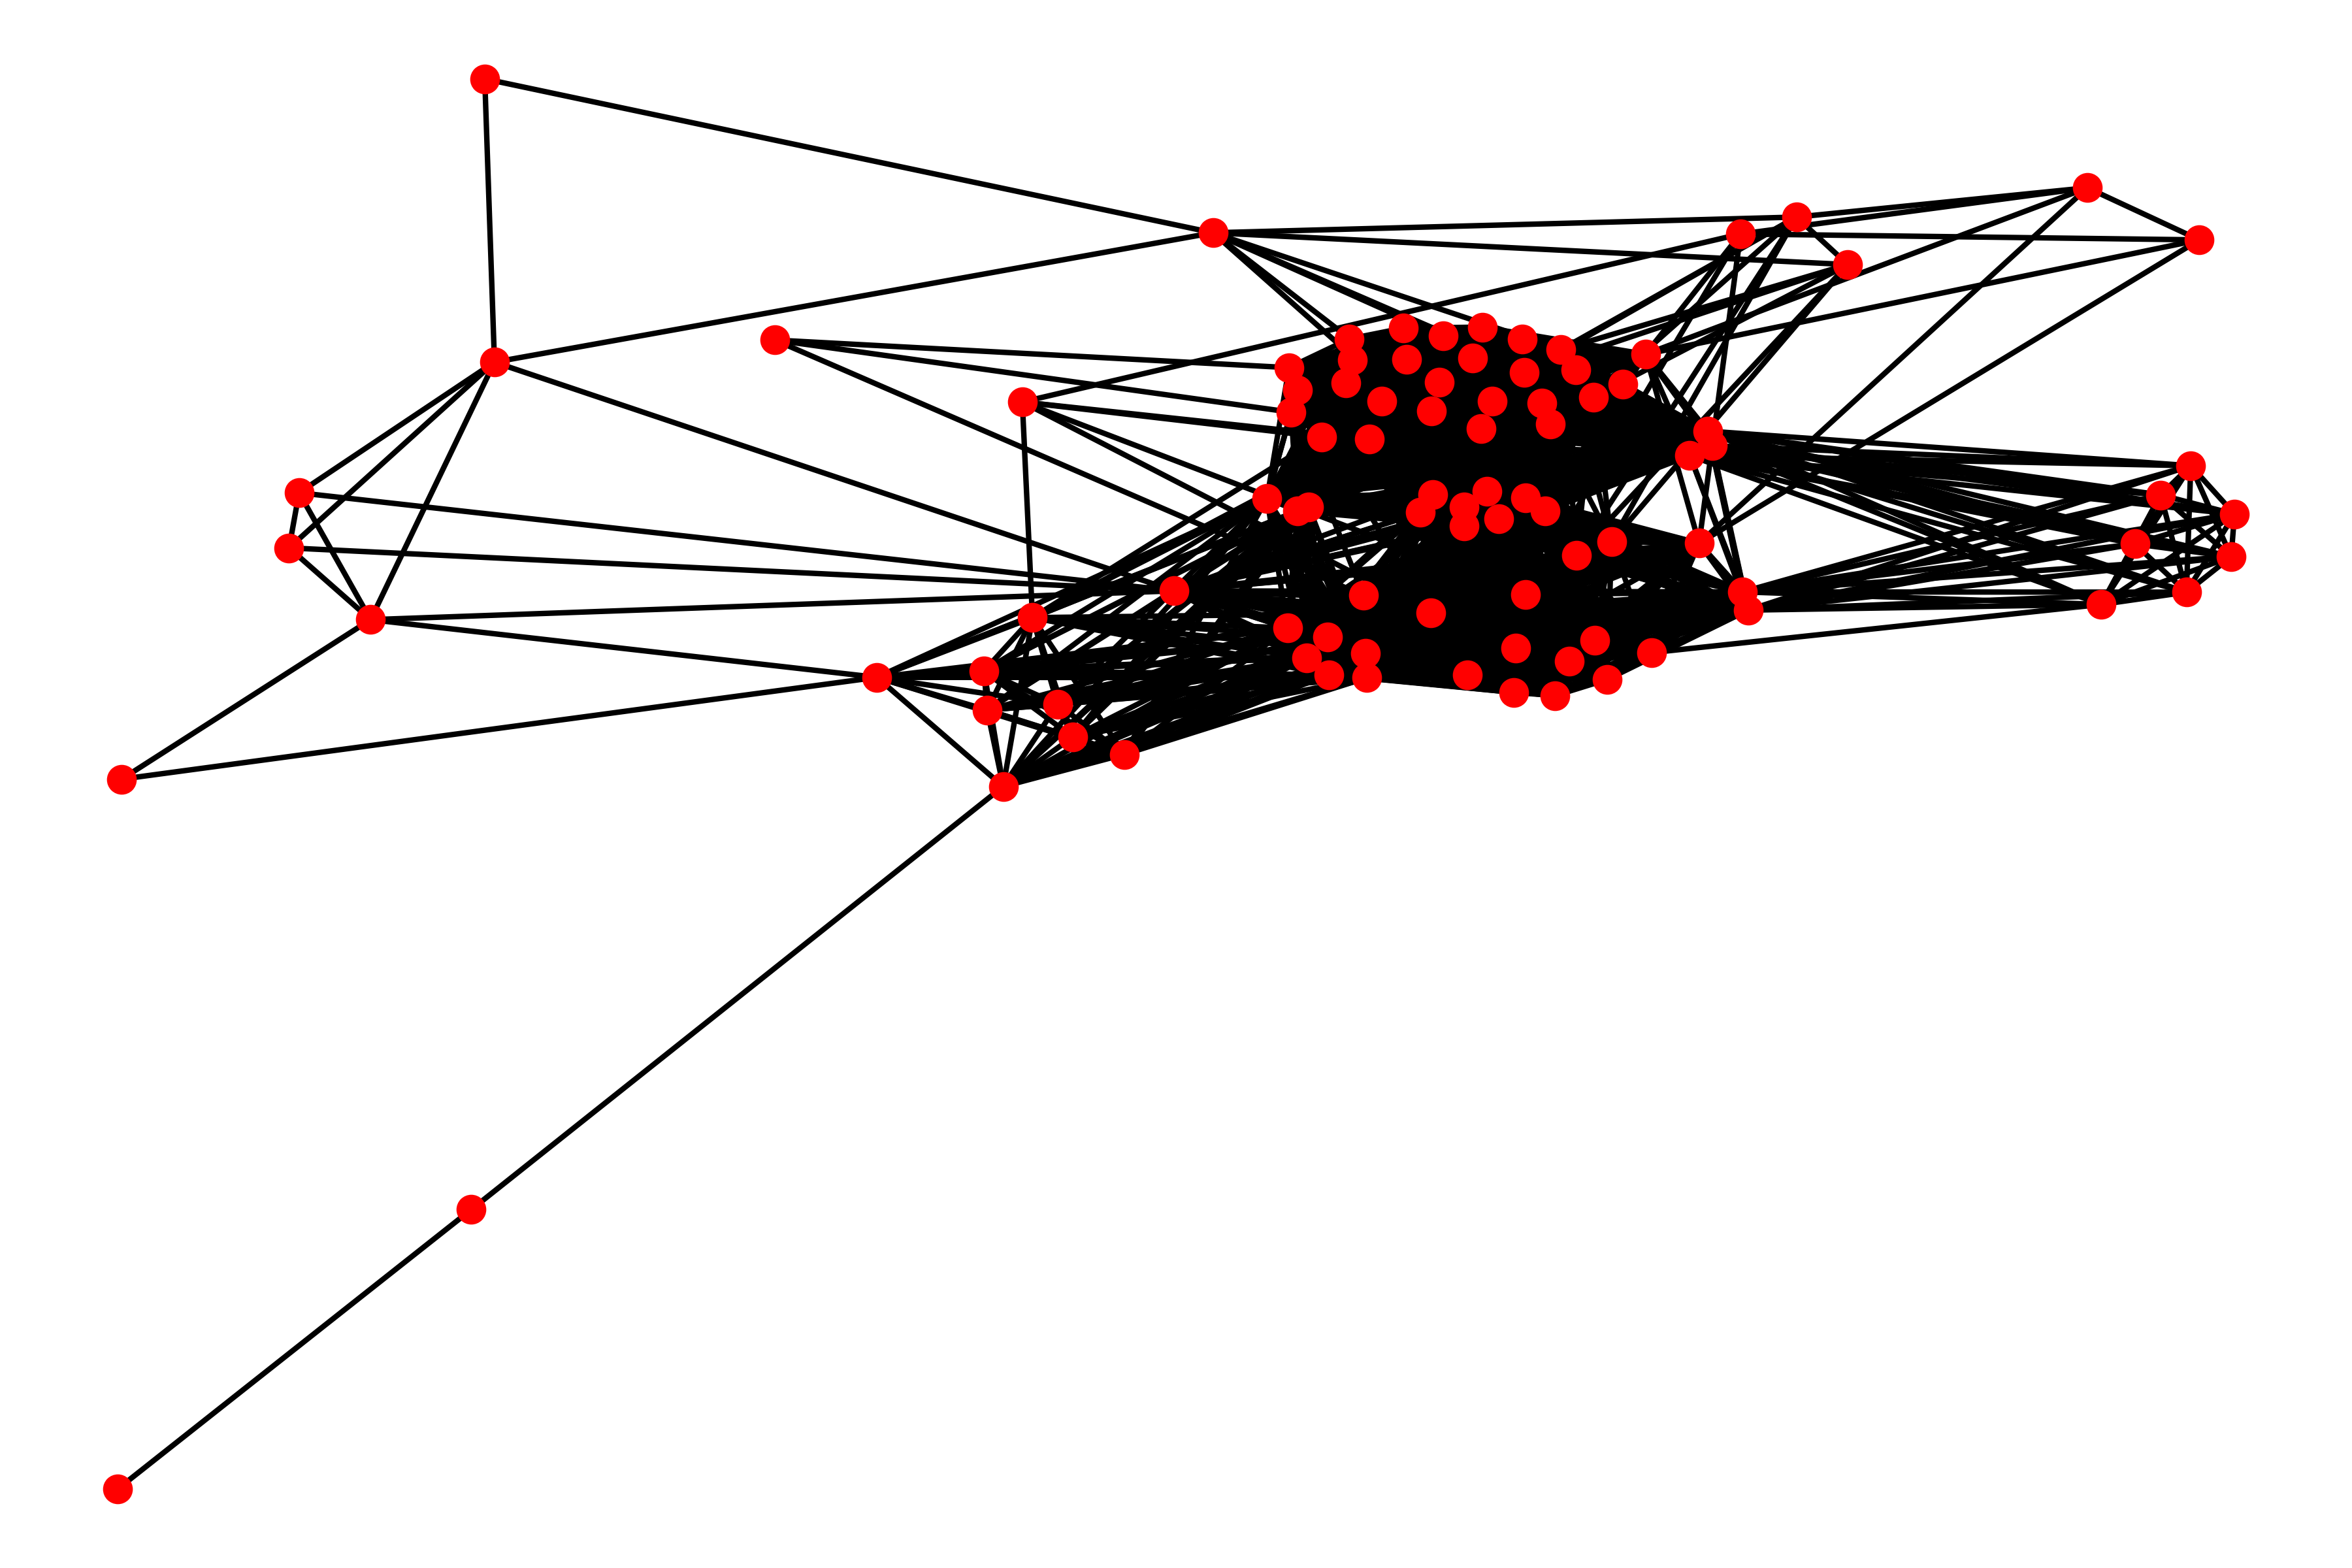
\includegraphics[width=\textwidth]{graphLineScaleFree.png}
        \caption{Line graph of scale free network}
        \label{fig:lineG}
    \end{subfigure}
    
    \begin{subfigure}[b]{\textwidth}
    	\begin{centering}
        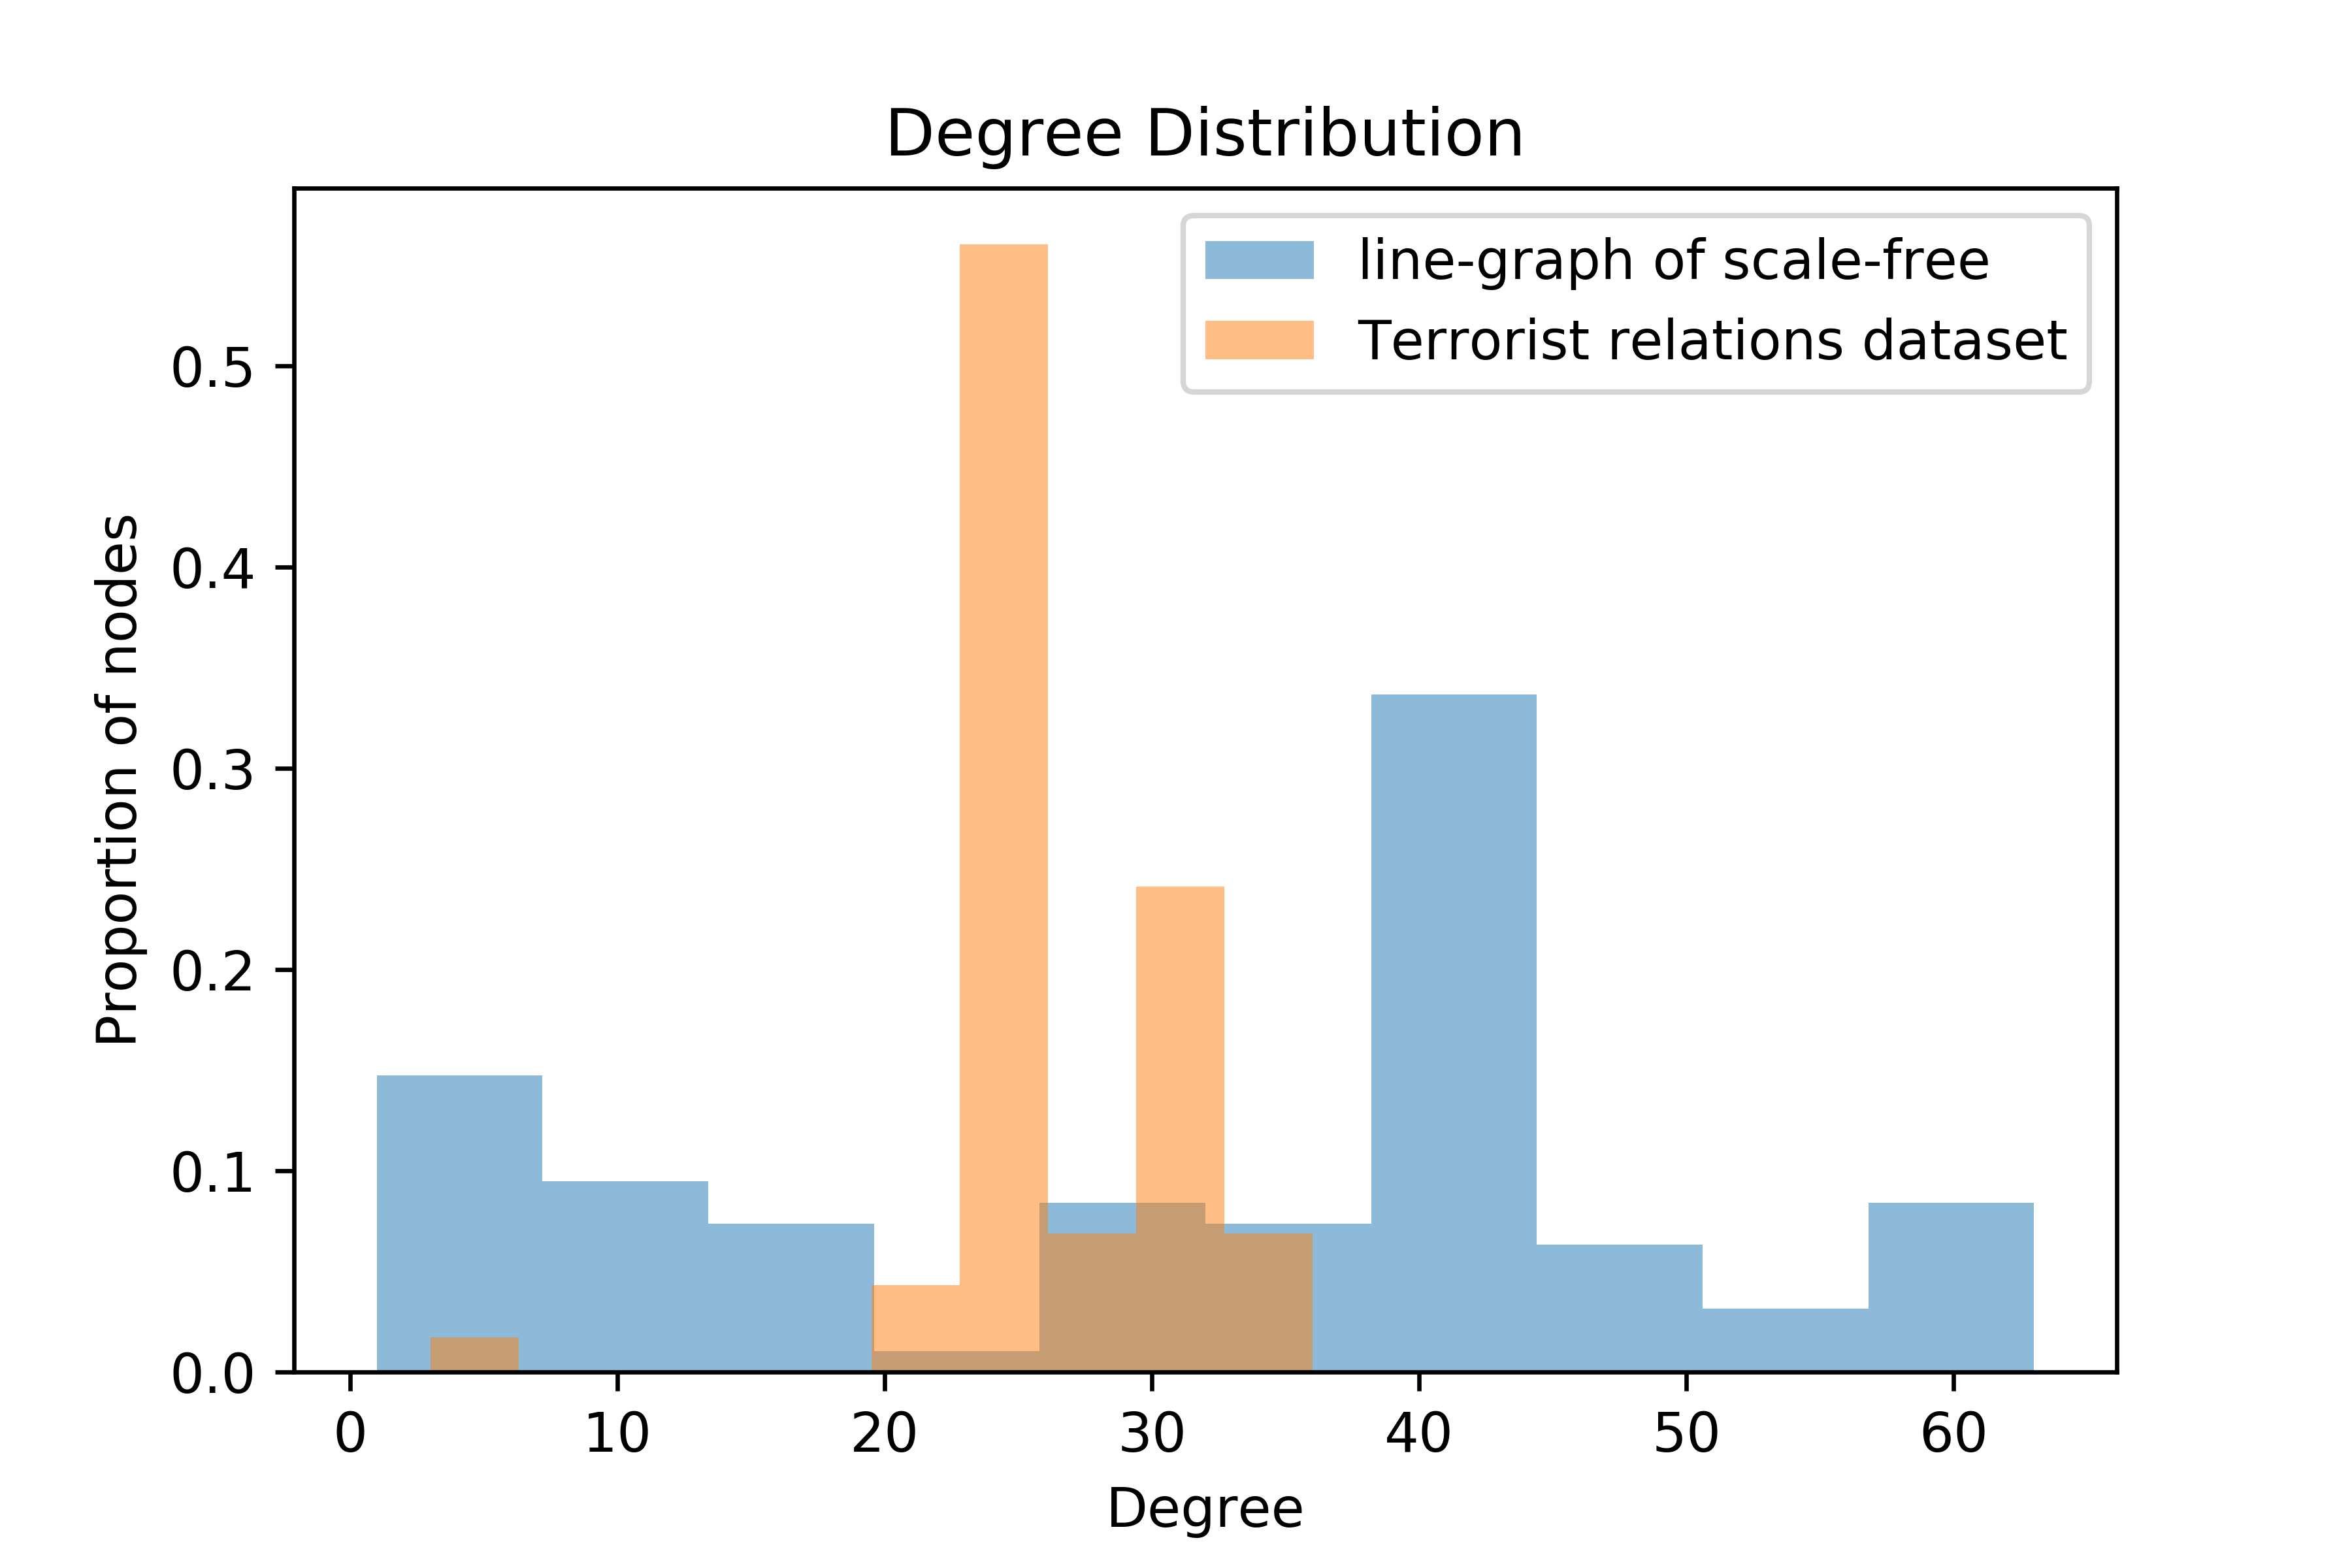
\includegraphics[width=.5\textwidth]{DegreeDiff.png}
        \caption{\centering Comparison of the degree distribution of the two line graphs. In blue, the created line graph and in orange the degrees of the relationships graph}
        \label{fig:DegDiff}
        \end{centering}
    \end{subfigure}
\caption{Graphs from the terror attacks dataset}
\label{fig:RelationshipScaleFree}
\end{center}
\end{figure}


\subsection{Terror Attacks Dataset}
\label{subsec:Terror Attacks Dataset}

\begin{figure}[H]
\begin{center}
    \begin{subfigure}[b]{0.45\textwidth}
        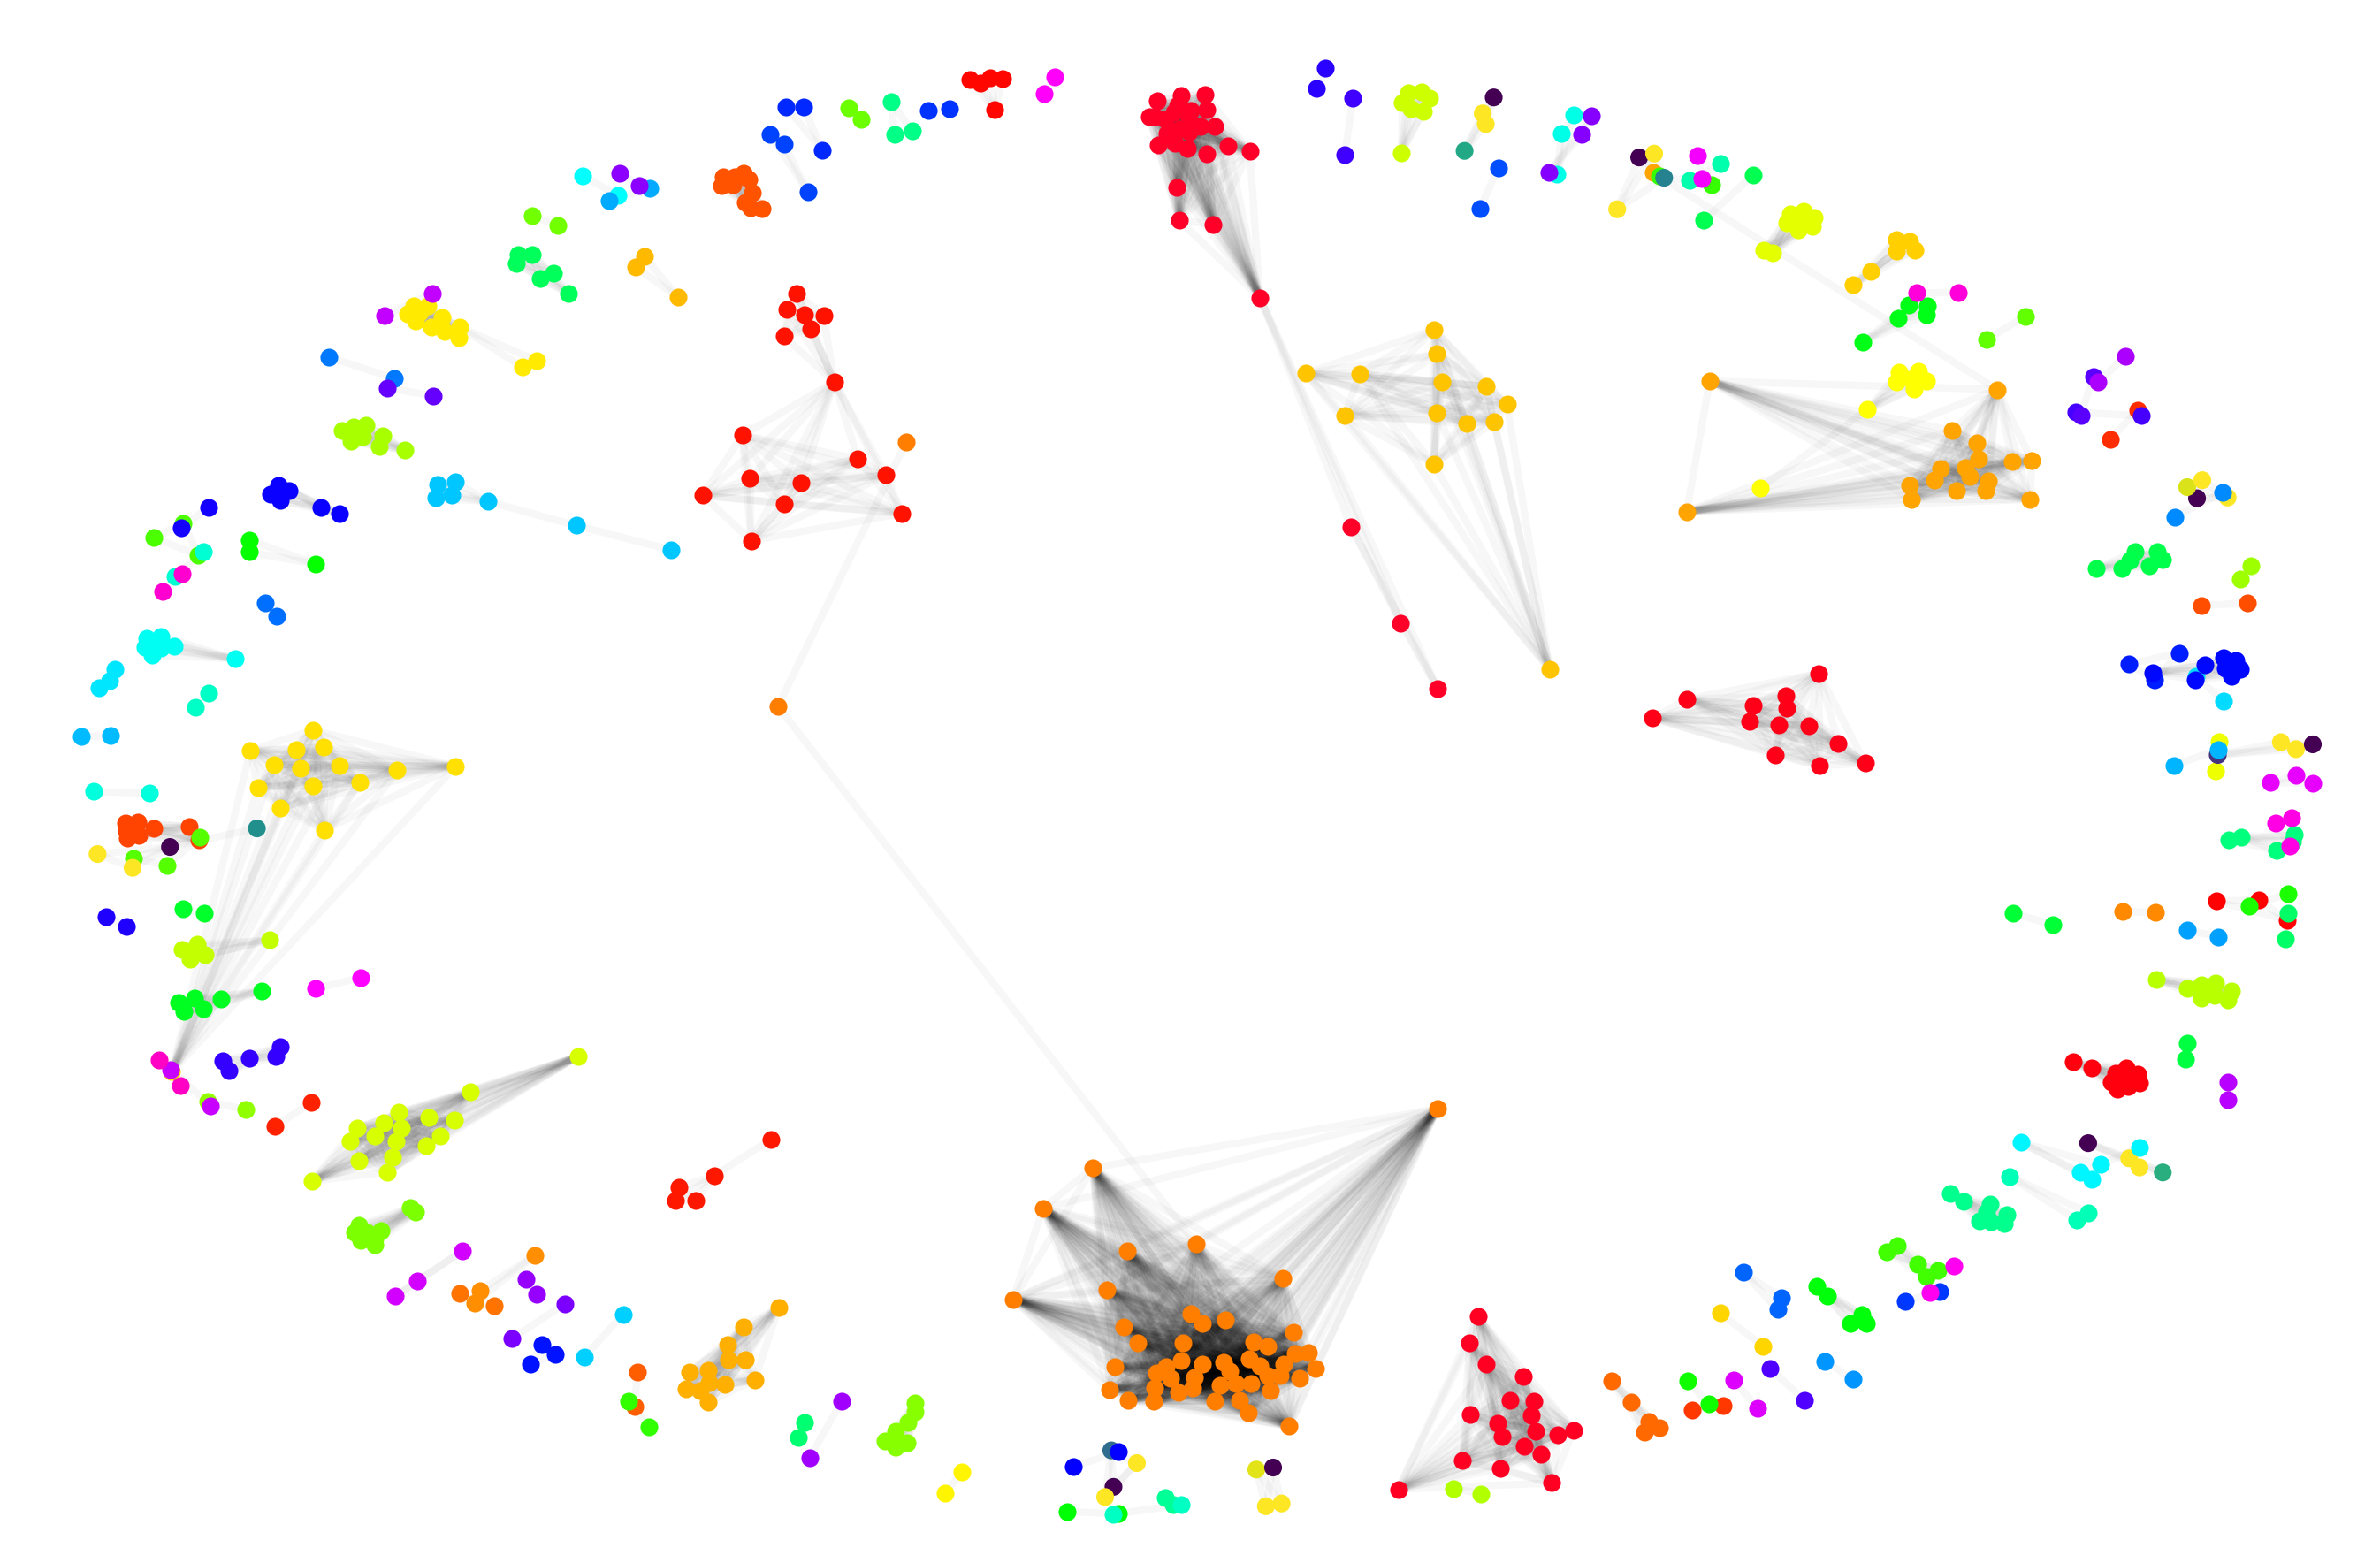
\includegraphics[width=\textwidth]{graphLoc.png}
        \caption{Terror attacks location graph, colouring by component ID}
        \label{fig:graphLoc}
    \end{subfigure}
    ~
    \begin{subfigure}[b]{0.45\textwidth}
        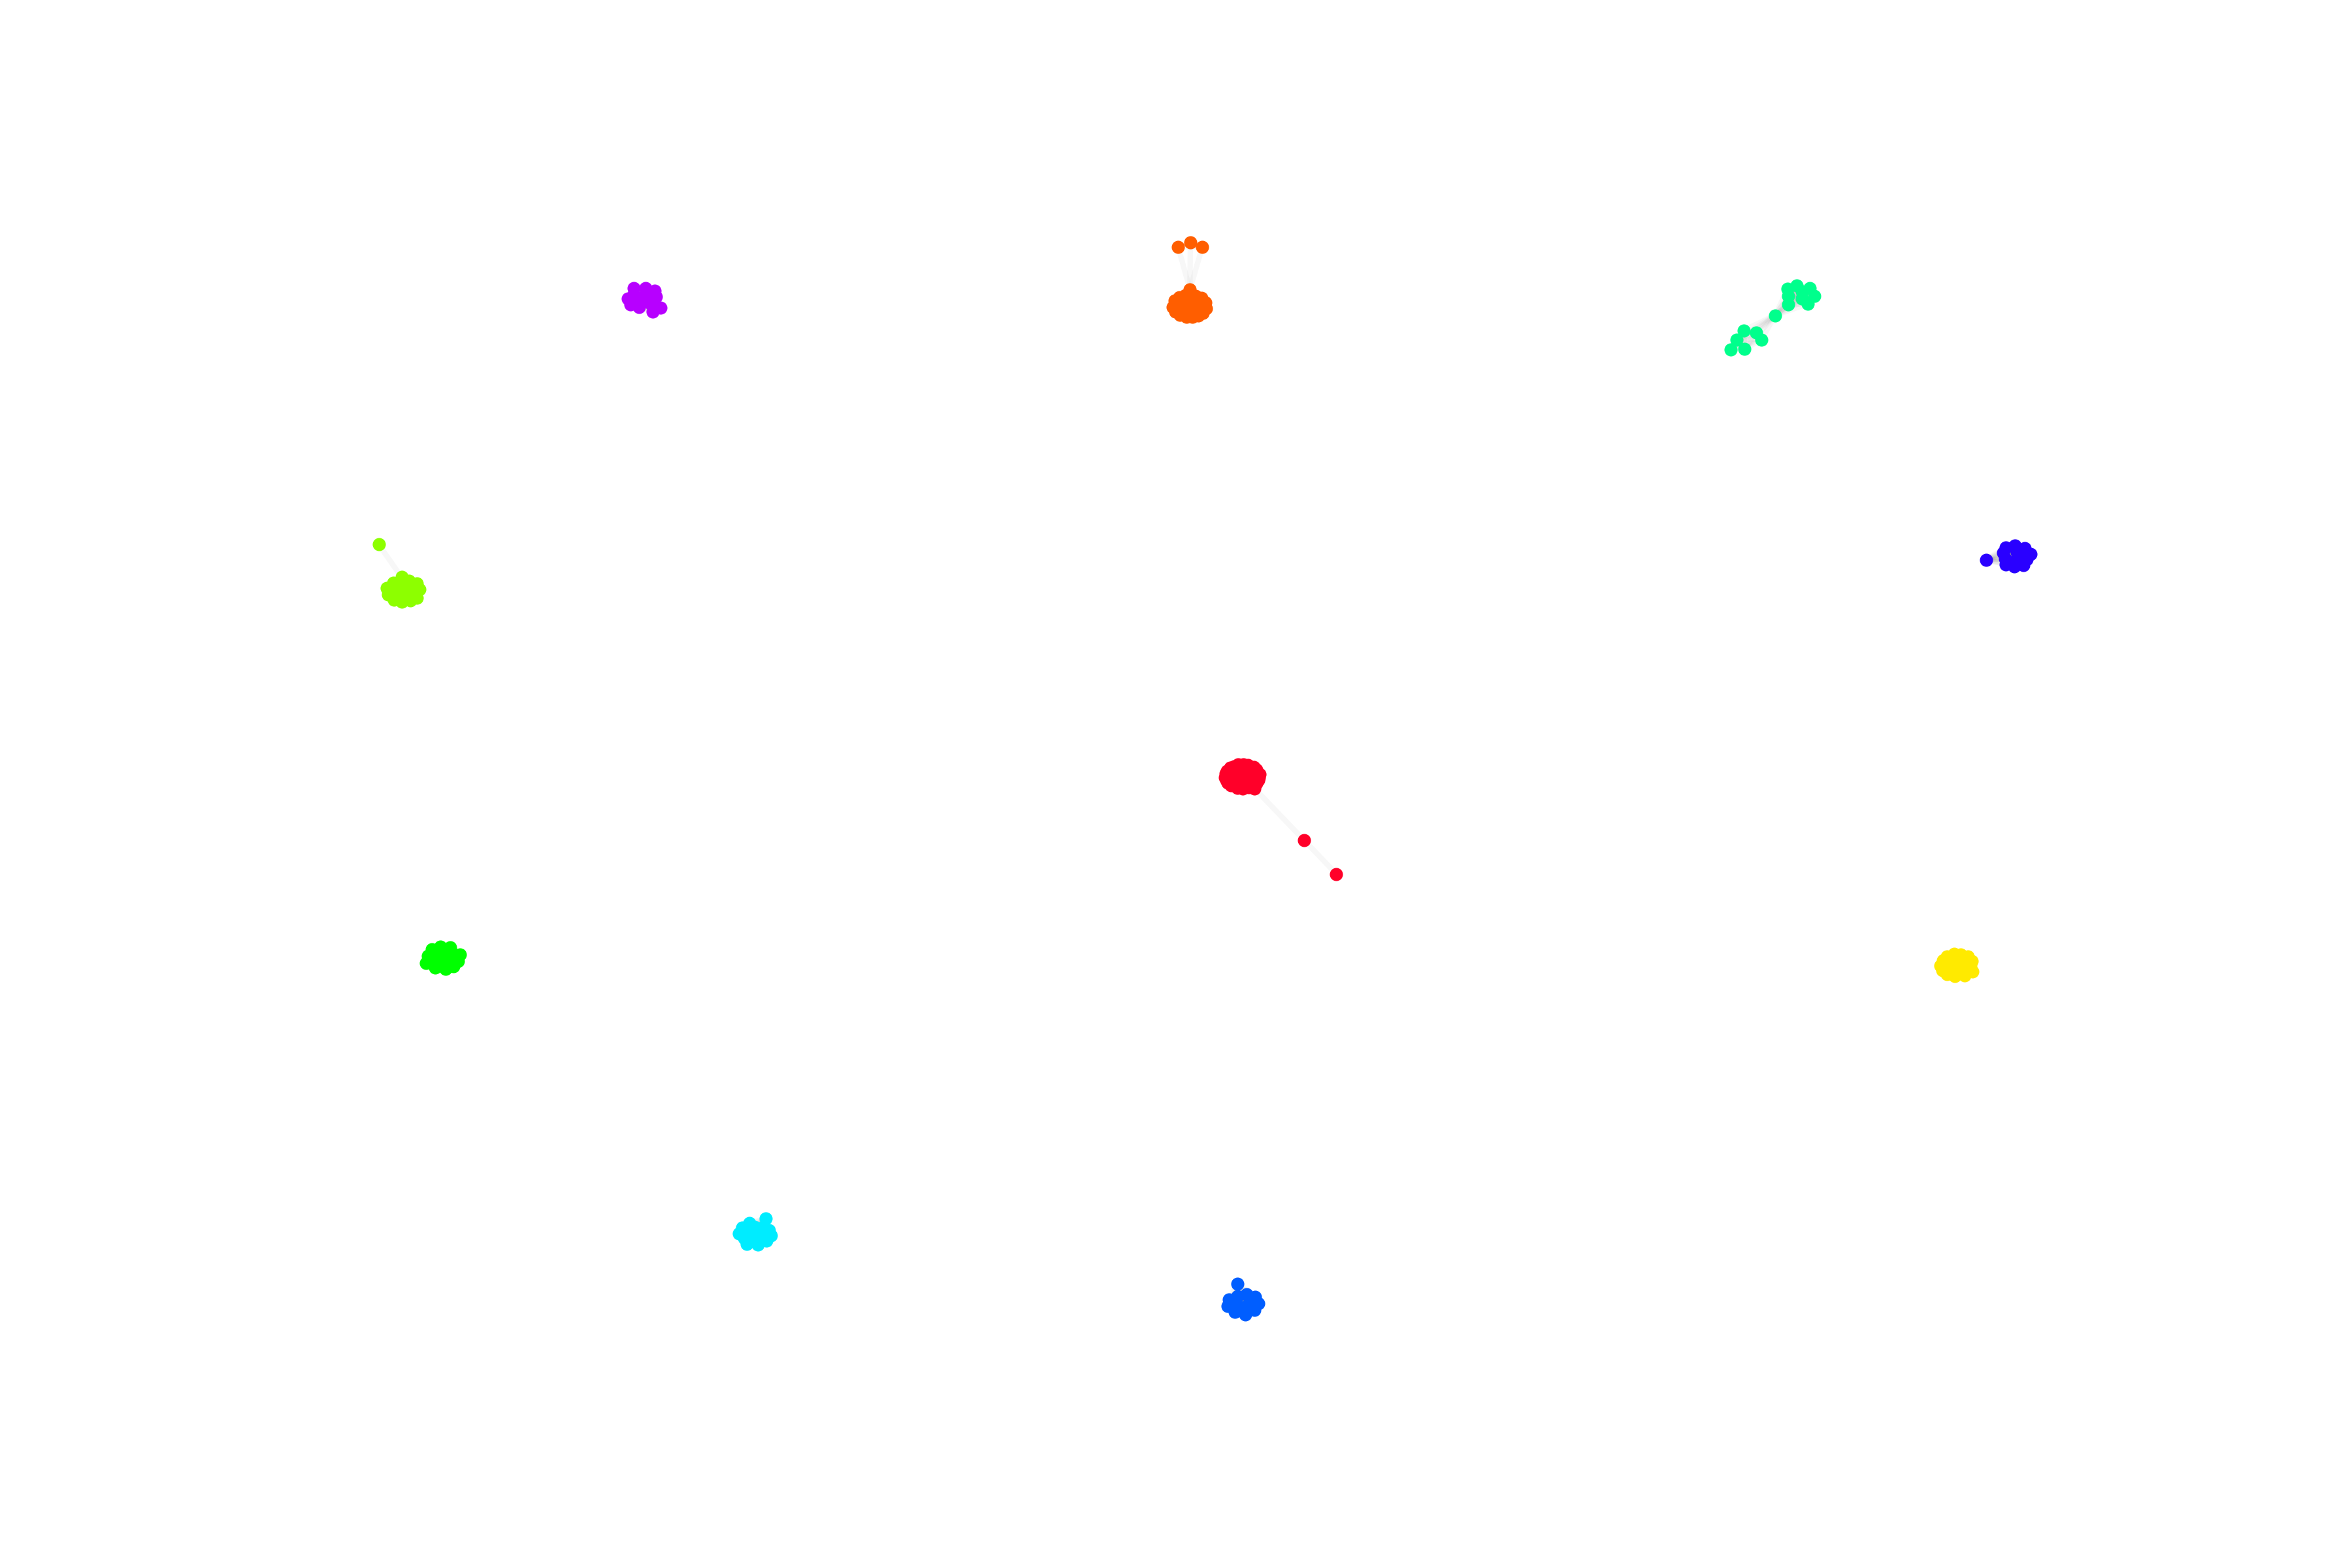
\includegraphics[width=\textwidth]{subGraph.png}
        \caption{Ten biggest components from the terror attacks location graph}
        \label{fig:subGraph}
    \end{subfigure}
\caption{Graphs from the terror attacks dataset}
\label{fig:graphPlots}
\end{center}
\end{figure}

Similarly to relationships datasets, we have found that the terrorist attacks dataset have very highly connected components, implying transitivity. 
If attack $a$ took place close to $b$, and attack $b$ took place close to $c$, then it is probable that attack $a$ took place close to $c$.

